\documentclass[12pt, a4paper]{article}

%% Кодировки и язык (для pdflatex)
\usepackage[utf8]{inputenc}
\usepackage[T2A]{fontenc}
\usepackage[russian, english]{babel}

%% Запасной вариант для отдельных Unicode-символов вне math-режима
\DeclareUnicodeCharacter{2208}{\ensuremath{\in}}
\DeclareUnicodeCharacter{221E}{\ensuremath{\infty}}
\DeclareUnicodeCharacter{2282}{\ensuremath{\subset}}

%% Математика
\usepackage{amsmath}
\usepackage{amssymb}
\let\Bbbk\relax
\usepackage{mathtools}
\usepackage{amsthm}
\newtheorem*{theorem}{Теорема}
\newtheorem*{lemma}{Лемма}

%% Поля
\usepackage[top=25mm, bottom=25mm, left=25mm, right=20mm]{geometry}
\usepackage{microtype}
\setlength{\parskip}{5pt plus 1pt}
\setlength{\parindent}{0pt}

%% Картинки
\usepackage{graphicx}

%% Макросы, которые обычно даёт шаблон pandoc (нужны при --to=latex)
\makeatletter
\newsavebox\pandoc@box
\newcommand*\pandocbounded[1]{%
  \sbox\pandoc@box{#1}%
  \Gscale@div\@tempa{\textheight}{\dimexpr\ht\pandoc@box+\dp\pandoc@box\relax}%
  \Gscale@div\@tempb{\linewidth}{\wd\pandoc@box}%
  \ifdim\@tempb\p@<\@tempa\p@\let\@tempa\@tempb\fi%
  \ifdim\@tempa\p@<\p@\else\gdef\@tempa{1}\fi%
  \scalebox{\@tempa}{\usebox\pandoc@box}%
}
\makeatother
\providecommand{\tightlist}{%
  \setlength{\itemsep}{0pt}\setlength{\parskip}{0pt}}

%% Гиперссылки + оглавление
\usepackage{hyperref}
\hypersetup{colorlinks=true, linkcolor=blue}

\title{Теория функций комплексного переменного\\[0.5em]
\large Вопросы к экзамену}
\author{karui}
\date{2025--2026}

\begin{document}
\maketitle
\tableofcontents
\newpage

    \section{Определение комплексного
числа}\label{ux43eux43fux440ux435ux434ux435ux43bux435ux43dux438ux435-ux43aux43eux43cux43fux43bux435ux43aux441ux43dux43eux433ux43e-ux447ux438ux441ux43bux430}

\textbf{Определение:} \emph{Комплексными числами} называются пары
\((x,y)\) действительных чисел \(x\) и \(y\), если для них определены
понятия равенства и операции сложения и умножения следующим образом:

\begin{enumerate}
\def\labelenumi{\arabic{enumi}.}
\tightlist
\item
  Два комплексных числа \((x_{1},y_{1})\) и \((x_{2},y_{2})\) считаются
  \emph{равными} тогда и только тогда, когда \(x_{1}=x_{2}\) и
  \(y_{1}=y_{2}\).
\item
  \emph{Суммой} двух комплексных чисел \((x_{1},y_{1})\) и
  \((x_{2},y_{2})\) называется комплексное число
  \((x_{1}+x_{2},y_{1}+y_{2})\).
\item
  \emph{Произведением} двух комплексных чисел \((x_{1},y_{1})\) и
  \((x_{2},y_{2})\) называется комплексное число
  \((x_{1}x_{2}-y_{1}y_{2},x_{1}y_{2}+x_{2}y_{1})\).
\end{enumerate}

Формулы: \[
(x_{1},y_{1})=(x_{2},y_{2})\text{, если } x_{1}=x_{2}\text{ и }y_{1}=y_{2}\quad(1)
\] \[
(x_{1},y_{1})+(x_{2},y_{2})=(x_{1}+x_{2},y_{1}+y_{2})\quad(2)
\] \[
(x_{1},y_{1})\cdot(x_{2},y_{2})=(x_{1}x_{2}-y_{1}y_{2},x_{1}y_{2}+x_{2}y_{1})\quad(3)
\]

\textbf{Определение:} Множество комплексных чисел, в котором введено
равенство, а также операции сложения и умножения, обозначают
\(\mathbb{C}\).

\textbf{Определение:} Комплексное число \((0,1)\) называют \emph{мнимой
единицей} и обозначается буквой \(i\). По формуле (3): \[
i^{2}=(0,1)\cdot(0,1)=(-1,0)=-1
\] Тогда по формулам (2) и (3): \[
(x,y)=(x,0)+(0,1)(y,0)=x+iy
\] Комплексные числа можно записать в алгебраической форме: \[
(x,y)=x+iy
\]

\textbf{Определение:} Комплексные числа вида \(0+iy\) называют
\emph{чисто мнимыми}.

Комплексное число \(x+iy\) принято обозначать одной буквой \(z\), т.е.
\(z=x+iy\). Число \(x\) называется \emph{действительной частью}, а число
\(y\) - \emph{мнимой частью} комплексного числа \(z=x+iy\). Для этих
чисел приняты следующие обозначения: \[
x=\mathrm{Re}(x+iy)=\mathrm{Re}z\quad y=\mathrm{Im}(x+iy)=\mathrm{Im}z
\]

\textbf{Определение:} Комплексное число \(x-iy\) называется
\emph{сопряженным} с комплексным числом \(z=x+iy\) и обозначается
\(\overline{z}\), т.е. \[
\overline{z}=\overline{x+iy}=x-iy
\]

\textbf{Определение:} Число \(\sqrt{ x^{2}+y^{2} }\) называется
\emph{модулем} комплексного числа \(z=x+iy\) и обозначается \(|z|\),
т.е. \[
|z|= |x+iy|=\sqrt{ x^{2}+y^{2} }
\] Соответствие между комплексными числами и точками плоскости является
взаимно однозначным. При этом действительные числа изображаются точками
оси абсцисс, а чисто мнимые --- точками оси ординат. Поэтому ось абсцисс
называется \emph{действительной осью}, а ось ординат - \emph{мнимой
осью}. Плоскость, на которой изображаются комплексные числа, называется
\emph{комплексной плоскостью}.

\textbf{Формы записей:}

\begin{enumerate}
\def\labelenumi{\arabic{enumi}.}
\tightlist
\item
  \(z=x+iy\) - алгебраическая
\item
  \(z=r(\cos \varphi+i\sin\varphi)\) - тригонометрическая,
\item
  \(z=re^{ i\varphi }\) - показательная, где \(r=|z|\), а
  \(\varphi=\arg z\) - угол между вектором \(z\) и положительным
  направлением действительной оси.
\end{enumerate}

\pandocbounded{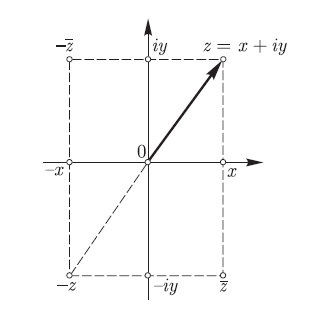
\includegraphics[keepaspectratio]{Вопросы/media/Pasted image 20260605151104.png}}

\newpage

\section{Определение расширенной комплексной плоскости. Описать алгоритм
построения сферы Римана. Сделать поясняющий
рисунок.}\label{ux43eux43fux440ux435ux434ux435ux43bux435ux43dux438ux435-ux440ux430ux441ux448ux438ux440ux435ux43dux43dux43eux439-ux43aux43eux43cux43fux43bux435ux43aux441ux43dux43eux439-ux43fux43bux43eux441ux43aux43eux441ux442ux438.-ux43eux43fux438ux441ux430ux442ux44c-ux430ux43bux433ux43eux440ux438ux442ux43c-ux43fux43eux441ux442ux440ux43eux435ux43dux438ux44f-ux441ux444ux435ux440ux44b-ux440ux438ux43cux430ux43dux430.-ux441ux434ux435ux43bux430ux442ux44c-ux43fux43eux44fux441ux43dux44fux44eux449ux438ux439-ux440ux438ux441ux443ux43dux43eux43a.}

\textbf{Определение:} Комплексная плоскость, дополненная бесконечно
удаленной точкой, называется \emph{расширенной комплексной плоскостью} и
обозначается \(\overline{\mathbb{C}}\), т.е. \[
\overline{\mathbb{C}}=\mathbb{C}\cup \{ \infty \}
\]

\subsubsection{Построение сферы Римана (стереографическая
проекция)}\label{ux43fux43eux441ux442ux440ux43eux435ux43dux438ux435-ux441ux444ux435ux440ux44b-ux440ux438ux43cux430ux43dux430-ux441ux442ux435ux440ux435ux43eux433ux440ux430ux444ux438ux447ux435ux441ux43aux430ux44f-ux43fux440ux43eux435ux43aux446ux438ux44f}

\begin{enumerate}
\def\labelenumi{\arabic{enumi}.}
\tightlist
\item
  Берём сферу \(S\), касающуюся комплексной плоскости \(\mathbb{C}\) в
  точке \(O\) (точка касания совпадает с началом координат).
\item
  Обозначаем через \(P\) точку сферы, диаметрально противоположную точке
  касания \(O\) (верхняя точка сферы).
\item
  Каждой точке \(z \in \mathbb{C}\) ставим в соответствие точку \(M\)
  --- точку пересечения сферы \(S\) с отрезком, соединяющим \(z\) и
  \(P\).
\item
  Это соответствие \(z \leftrightarrow M\) между точками плоскости и
  точками сферы (кроме \(P\)) взаимно однозначно.
\item
  Единственная точка сферы, не имеющая прообраза на плоскости, --- сам
  полюс \(P\). Последовательности \(\{z_n\}\) с \(|z_n| \to \infty\)
  соответствует последовательность точек сферы, сходящаяся к \(P\).
  Поэтому точке \(z = \infty\) ставят в соответствие \(P\).
\end{enumerate}

\subsubsection{Формулы стереографической проекции
(опционально)}\label{ux444ux43eux440ux43cux443ux43bux44b-ux441ux442ux435ux440ux435ux43eux433ux440ux430ux444ux438ux447ux435ux441ux43aux43eux439-ux43fux440ux43eux435ux43aux446ux438ux438-ux43eux43fux446ux438ux43eux43dux430ux43bux44cux43dux43e}

Введём координаты: плоскость \(\mathbb{C}\) --- это плоскость
\(\{w = 0\}\) в пространстве \((u, v, w)\), где точке \(z = x + iy\)
отвечает \((x, y, 0)\). Сферу \(S\), касающуюся плоскости в точке \(O\),
зададим уравнением

\[u^2 + v^2 + \left(w - \tfrac12\right)^2 = \tfrac14\]

(радиус \(\tfrac12\), нижняя точка --- \(O = (0,0,0)\), полюс ---
\(P = (0,0,1)\)).

Тогда соответствие \(z \leftrightarrow M\) из алгоритма выписывается в
координатах явно. Точке \(z\) отвечает точка \(M = (u, v, w)\) сферы:

\[u = \frac{x}{1+|z|^2}, \quad v = \frac{y}{1+|z|^2}, \quad w = \frac{|z|^2}{1+|z|^2};\]

обратно, по точке \(M\) восстанавливается \(z\):

\[x = \frac{u}{1-w}, \quad y = \frac{v}{1-w}.\]

Эти формулы делают взаимную однозначность соответствия
\(z \leftrightarrow M\) явной. При \(|z| \to \infty\) получаем
\(w \to 1\), то есть точка \(M\) стремится к полюсу \(P\) --- что
согласуется с сопоставлением \(z = \infty \leftrightarrow P\) из пункта
5.

\textbf{Определение:} соответствие между точками расширенной комплексной
плоскости \(\overline{\mathbb{C}} = \mathbb{C} \cup \{\infty\}\) и
точками сферы \(S\) взаимно однозначно. Сфера \(S\) с таким
соответствием называется \textbf{сферой Римана}.

\pandocbounded{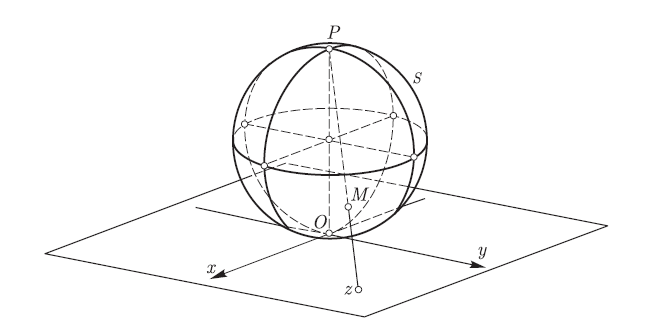
\includegraphics[keepaspectratio]{Вопросы/media/Pasted image 20260605161528.png}}

\newpage

\section{Определение предельной точки и предела последовательности из
комплексных чисел. Необходимое и достаточное условие сходимости
последовательности (сходимость действительных и мнимых частей).
Определение бесконечно большой последовательности из комплексных
чисел.}\label{ux43eux43fux440ux435ux434ux435ux43bux435ux43dux438ux435-ux43fux440ux435ux434ux435ux43bux44cux43dux43eux439-ux442ux43eux447ux43aux438-ux438-ux43fux440ux435ux434ux435ux43bux430-ux43fux43eux441ux43bux435ux434ux43eux432ux430ux442ux435ux43bux44cux43dux43eux441ux442ux438-ux438ux437-ux43aux43eux43cux43fux43bux435ux43aux441ux43dux44bux445-ux447ux438ux441ux435ux43b.-ux43dux435ux43eux431ux445ux43eux434ux438ux43cux43eux435-ux438-ux434ux43eux441ux442ux430ux442ux43eux447ux43dux43eux435-ux443ux441ux43bux43eux432ux438ux435-ux441ux445ux43eux434ux438ux43cux43eux441ux442ux438-ux43fux43eux441ux43bux435ux434ux43eux432ux430ux442ux435ux43bux44cux43dux43eux441ux442ux438-ux441ux445ux43eux434ux438ux43cux43eux441ux442ux44c-ux434ux435ux439ux441ux442ux432ux438ux442ux435ux43bux44cux43dux44bux445-ux438-ux43cux43dux438ux43cux44bux445-ux447ux430ux441ux442ux435ux439.-ux43eux43fux440ux435ux434ux435ux43bux435ux43dux438ux435-ux431ux435ux441ux43aux43eux43dux435ux447ux43dux43e-ux431ux43eux43bux44cux448ux43eux439-ux43fux43eux441ux43bux435ux434ux43eux432ux430ux442ux435ux43bux44cux43dux43eux441ux442ux438-ux438ux437-ux43aux43eux43cux43fux43bux435ux43aux441ux43dux44bux445-ux447ux438ux441ux435ux43b.}

\textbf{Определение:} \(\{ z_{n} \}\) - последовательность в
\(\mathbb{C}\).

\textbf{Определение:} Точка \(b \in \mathbb{C}\) называется
\emph{предельной точкой} последовательности \(\{z_n\}\), если
\[\forall \delta > 0 \;\; \forall N \in \mathbb{N} \;\; \exists n > N: \; z_n \in \dot{U}_\delta(b).\]

\textbf{Определение:} \(\mathcal{B}\) - множество предельных точек
последовательности.

\textbf{Определение:} \(A=\lim_{ n \to \infty }z_{n}\), если
\(\mathcal{B}=\{ A \}\) - единственная предельная точка \[
\forall\varepsilon>0 \ \exists n_{\mathcal{E}}: \ \forall n\geq n_{\mathcal{E}} \to |z_{n}-A|<\varepsilon\Leftrightarrow  z_{n}\in U_{\varepsilon}(A)
\]

\textbf{Теорема:} (Необходимое и достаточное условие сходимости
последовательности) Последовательность
\(\{ z_{n} \}, \ z_{n}=a_{n}+ib_{n}\) имеет предел равный \(A=a+bi\) в
том и только в том случае, если \(\exists \lim_{ n \to \infty }a_{n}=a\)
и \(\exists \lim_{ n \to \infty }b_{n}=b\).

\textbf{Определение:}
\(\lim_{ n \to \infty }z_{n}=\infty\Leftrightarrow\forall R>0 \ \exists N: \forall n\geq N\to |z_{n}|>R\).

\newpage

\section{Определение ряда из комплексных чисел. Определение сходящегося
ряда. Связь со сходимостью рядов действительной и мнимой
частей.}\label{ux43eux43fux440ux435ux434ux435ux43bux435ux43dux438ux435-ux440ux44fux434ux430-ux438ux437-ux43aux43eux43cux43fux43bux435ux43aux441ux43dux44bux445-ux447ux438ux441ux435ux43b.-ux43eux43fux440ux435ux434ux435ux43bux435ux43dux438ux435-ux441ux445ux43eux434ux44fux449ux435ux433ux43eux441ux44f-ux440ux44fux434ux430.-ux441ux432ux44fux437ux44c-ux441ux43e-ux441ux445ux43eux434ux438ux43cux43eux441ux442ux44cux44e-ux440ux44fux434ux43eux432-ux434ux435ux439ux441ux442ux432ux438ux442ux435ux43bux44cux43dux43eux439-ux438-ux43cux43dux438ux43cux43eux439-ux447ux430ux441ux442ux435ux439.}

\textbf{Определение:} Пусть \(\{z_n\}\), \(z_n \in \mathbb{C}\).
Числовой ряд:
\[\sum_{n=1}^{\infty} z_n = z_1 + z_2 + \dots, \qquad z_n \text{ — общий член.}\]

\textbf{Определение:} Частичная сумма:
\[S_n = \sum_{k=1}^{n} z_k, \qquad \{S_n\} \text{ — последовательность частичных сумм.}\]

\textbf{Определение:} Ряд \(\sum z_n\) сходится
\(\;\Leftrightarrow\; \exists\, S \in \mathbb{C}:\)
\[\forall \varepsilon > 0 \;\; \exists n_\varepsilon \;\; \forall n \geq n_\varepsilon : \; |S_n - S| < \varepsilon.\]
\(S = \lim\limits_{n\to\infty} S_n = \sum\limits_{n=1}^{\infty} z_n\)
--- сумма ряда. Иначе ряд расходится.

\textbf{Теорема (связь с Re/Im):} \(z_n = a_n + i b_n\),
\(\;a_n, b_n \in \mathbb{R}\):
\[\sum_{n=1}^{\infty} z_n \text{ сходится} \;\;\Longleftrightarrow\;\; \exists \sum_{n=1}^{\infty} a_n \;\wedge\; \exists \sum_{n=1}^{\infty} b_n,\]
\[\sum_{n=1}^{\infty} z_n = \sum_{n=1}^{\infty} a_n + i \sum_{n=1}^{\infty} b_n.\]

\newpage

\section{Определение абсолютно сходящегося ряда. Критерий Коши для рядов
комплексных
чисел.}\label{ux43eux43fux440ux435ux434ux435ux43bux435ux43dux438ux435-ux430ux431ux441ux43eux43bux44eux442ux43dux43e-ux441ux445ux43eux434ux44fux449ux435ux433ux43eux441ux44f-ux440ux44fux434ux430.-ux43aux440ux438ux442ux435ux440ux438ux439-ux43aux43eux448ux438-ux434ux43bux44f-ux440ux44fux434ux43eux432-ux43aux43eux43cux43fux43bux435ux43aux441ux43dux44bux445-ux447ux438ux441ux435ux43b.}

\textbf{Определение:} Говорят, что ряд
\(\sum\limits_{n=1}^{\infty}z_{n}\) сходится \emph{абсолютно}, если
\(\sum\limits_{n=1}^{\infty}|z_{n}|\) сходится.

\textbf{Теорема:} (Критерий Коши для рядов комплексных чисел) \[
\forall\varepsilon>0 \ \exists n_{\varepsilon}: \ \forall m,n\geq n_{\varepsilon}\implies |\underbrace{z_{m+1}+z_{m+2}+\dots+z_{n}}_{S_{n}-S_{m}}|<\varepsilon
\] это необходимое и достаточное условие сходимости ряда.

\newpage

\section{\texorpdfstring{Определение области. Определение функции
комплексного переменного, заданной на области
\(G \subset \mathbb{C}\).}{Определение области. Определение функции комплексного переменного, заданной на области G \textbackslash subset \textbackslash mathbb\{C\}.}}\label{ux43eux43fux440ux435ux434ux435ux43bux435ux43dux438ux435-ux43eux431ux43bux430ux441ux442ux438.-ux43eux43fux440ux435ux434ux435ux43bux435ux43dux438ux435-ux444ux443ux43dux43aux446ux438ux438-ux43aux43eux43cux43fux43bux435ux43aux441ux43dux43eux433ux43e-ux43fux435ux440ux435ux43cux435ux43dux43dux43eux433ux43e-ux437ux430ux434ux430ux43dux43dux43eux439-ux43dux430-ux43eux431ux43bux430ux441ux442ux438-g-subset-mathbbc.}

\textbf{Определение:} Окрестность точки \(z_{0}\): \[
U_{\delta}(z_{0})=\{ z\in \mathbb{C}:|z-z_{0}|<\delta \}
\] \textbf{Определение:} Окрестность \(\infty\): \[
U_{R}(\infty)=\{ z\in \mathbb{C}:|z|>R \}
\]

\textbf{Определение:} Множество \(G \subset \overline{\mathbb{C}}\)
называется связным, если \(\forall z_1, z_2 \in G\ \exists\) непрерывная
кривая \(\gamma \subset G\), соединяющая \(z_{1}\) и \(z_2\).

\textbf{Определение:} Множество \(G\subset \overline{\mathbb{C}}\)
называется открытым, если
\(\forall z_{0}\in G \ \ \exists U(z_{0})\subset G\)

\textbf{Определение:} \(G\) - область в \(\overline{\mathbb{C}}\) - это
открытое, связное множество.

\textbf{Определение:} Функция комплексного переменного:
\(w=f(z), \ z\in G \overset{f}{\to}w\in f(G)\subset \mathbb{C}\). \[
z=x+iy, \quad w=u(x,y)+i\cdot v(x,y), \quad u=\mathrm{Re}f(z), \ v=\mathrm{Im}f(z)
\]

\newpage

\section{Определение предела функции в точке области. Связь с
существованием пределов действительной и мнимой части функции.
Определение непрерывной функции в точке и в
области.}\label{ux43eux43fux440ux435ux434ux435ux43bux435ux43dux438ux435-ux43fux440ux435ux434ux435ux43bux430-ux444ux443ux43dux43aux446ux438ux438-ux432-ux442ux43eux447ux43aux435-ux43eux431ux43bux430ux441ux442ux438.-ux441ux432ux44fux437ux44c-ux441-ux441ux443ux449ux435ux441ux442ux432ux43eux432ux430ux43dux438ux435ux43c-ux43fux440ux435ux434ux435ux43bux43eux432-ux434ux435ux439ux441ux442ux432ux438ux442ux435ux43bux44cux43dux43eux439-ux438-ux43cux43dux438ux43cux43eux439-ux447ux430ux441ux442ux438-ux444ux443ux43dux43aux446ux438ux438.-ux43eux43fux440ux435ux434ux435ux43bux435ux43dux438ux435-ux43dux435ux43fux440ux435ux440ux44bux432ux43dux43eux439-ux444ux443ux43dux43aux446ux438ux438-ux432-ux442ux43eux447ux43aux435-ux438-ux432-ux43eux431ux43bux430ux441ux442ux438.}

Пусть функция \(f(z)\) определена в проколотой окрестности точки
\(z_0\), т.е. в кольце \[K: 0 < |z - z_0| < R.\] \textbf{Определение
предела по Коши:} Комплексное число \(A\) называется пределом функции
\(f(z)\) при \(z \to z_0\), если
\[\forall \varepsilon > 0\ \exists \delta > 0: \forall z,\ 0 < |z - z_0| < \delta \Rightarrow |f(z) - A| < \varepsilon.\]
Обозначение: \(\lim\limits_{z \to z_0} f(z) = A\), или \(f(z) \to A\)
при \(z \to z_0\).

\textbf{Определение предела по Гейне:} Комплексное число \(A\)
называется пределом функции \(f(z)\) в точке \(z_0\), если для любой
последовательности \(\{z_n\}\), \(z_n \in K\), сходящейся к \(z_0\),
последовательность \(\{f(z_n)\}\) сходится к \(A\):
\[\forall \{z_n\},\ z_n \in K,\ \lim_{n\to\infty} z_n = z_0 \;\Rightarrow\; \lim_{n\to\infty} f(z_n) = A.\]
Определения по Коши и по Гейне эквивалентны.

\textbf{Теорема (связь с Re/Im):} Пусть \(f(z) = u(x,y) + i\,v(x,y)\),
\(z_0 = x_0 + i y_0\). Существование предела
\(\lim\limits_{z \to z_0} f(z)\) равносильно существованию двух пределов
\(\lim\limits_{\substack{x \to x_0 \\ y \to y_0}} u(x,y)\) и
\(\lim\limits_{\substack{x \to x_0 \\ y \to y_0}} v(x,y)\), причём
\[\lim_{z \to z_0} f(z) = \lim_{\substack{x \to x_0 \\ y \to y_0}} u(x,y) + i \lim_{\substack{x \to x_0 \\ y \to y_0}} v(x,y).\]

\textbf{Определение:} \emph{Непрерывность функции:}

\begin{enumerate}
\def\labelenumi{\arabic{enumi}.}
\tightlist
\item
  в точке
  \(z=z_{0}\Leftrightarrow \lim\limits_{ z \to z_{0} }f(z)=f(z_{0})\Leftrightarrow\Delta f=f(z_{0}+\Delta z)-f(z_{0})=o(1)\Leftrightarrow \lim\limits_{ \Delta z \to 0 }\Delta f=0\)
\item
  В области \(G\) \(\Leftrightarrow f(z)\) непрерывна в
  \(\forall z_{0}\in G\)
\item
  в замкнутой области \(\overline{G}\) - непрерывная \(\forall z_{0}\)
  внутренних + \(\forall z_{0}\in\partial G\)
\end{enumerate}

\textbf{Утверждение 1:} \(f(z)=u(x,y)+i\cdot v(x,y), \ z=x+iy\)
Непрерывность функции \(f(z)\) по определению выше \(\Leftrightarrow\)
непрерывность функций \(u(x,y)\) и \(v(x,y)\) по пунктам из определения
непрерывности.

\newpage

\section{\texorpdfstring{Определение равномерно сходящегося
функционального ряда в области \(G \subset \mathbb{C}\). Достаточный
признак Вейерштрасса равномерной сходимости функционального
ряда}{Определение равномерно сходящегося функционального ряда в области G \textbackslash subset \textbackslash mathbb\{C\}. Достаточный признак Вейерштрасса равномерной сходимости функционального ряда}}\label{ux43eux43fux440ux435ux434ux435ux43bux435ux43dux438ux435-ux440ux430ux432ux43dux43eux43cux435ux440ux43dux43e-ux441ux445ux43eux434ux44fux449ux435ux433ux43eux441ux44f-ux444ux443ux43dux43aux446ux438ux43eux43dux430ux43bux44cux43dux43eux433ux43e-ux440ux44fux434ux430-ux432-ux43eux431ux43bux430ux441ux442ux438-g-subset-mathbbc.-ux434ux43eux441ux442ux430ux442ux43eux447ux43dux44bux439-ux43fux440ux438ux437ux43dux430ux43a-ux432ux435ux439ux435ux440ux448ux442ux440ux430ux441ux441ux430-ux440ux430ux432ux43dux43eux43cux435ux440ux43dux43eux439-ux441ux445ux43eux434ux438ux43cux43eux441ux442ux438-ux444ux443ux43dux43aux446ux438ux43eux43dux430ux43bux44cux43dux43eux433ux43e-ux440ux44fux434ux430}

\textbf{Определение:} Функциональные ряды:
\(\sum f_{n}(z), \ f_{n}(z)=u_{n}(x,y)+i\cdot v(x,y)\),
\(\sum u_{n}(x,y), \ \sum v_{n}(x,y)\). \textbf{Определение:}
\(S_{n}=\sum\limits_{k=1}^{n}f_{k}(z)\) - частичная сумма,
\(\mathrm{Re} S_{n}(z)=\sum\limits_{k=1}^{n}u_{k}(x,y), \quad \mathrm{Im} S_{n}(z)=\sum\limits_{k=1}^{n}v_{k}(x,y)\)

\textbf{Определение:} Сходимость ряда равномерная по области
\(G\subset \mathbb{C}\Leftrightarrow\)
\(S_{n}(z)\overset{G}{\underset{n\to \infty}{\rightrightarrows}}S(z)\Leftrightarrow\)
\[
\forall\varepsilon>0 \ \exists n_{\varepsilon}: \ \forall n\geq n_{\varepsilon} \ \forall z\in G \implies |S_{n}(z)-S(z)|<\varepsilon
\]

\textbf{Теорема:} (Достаточный признак Вейерштрасса равномерной
сходимости функционального ряда). Пусть
\(\exists \sum u_{n}, \ u_{n}\in \mathbb{C}\):

\begin{enumerate}
\def\labelenumi{\arabic{enumi}.}
\tightlist
\item
  \(|f_{n}(z)|\leq |u_{n}|, \ \forall n\geq n_{0}, \ \forall z\in G\)\\
\item
  \(\sum |u_{n}|\) сходится Тогда ряд \(\sum f_{n}(z)\) сходится на
  \(G\) равномерно.
\end{enumerate}

\newpage

\section{Понятие производной функции комплексного переменного в точке и
её дифференцируемости. Необходимые и достаточные условия
дифференцируемости.}\label{ux43fux43eux43dux44fux442ux438ux435-ux43fux440ux43eux438ux437ux432ux43eux434ux43dux43eux439-ux444ux443ux43dux43aux446ux438ux438-ux43aux43eux43cux43fux43bux435ux43aux441ux43dux43eux433ux43e-ux43fux435ux440ux435ux43cux435ux43dux43dux43eux433ux43e-ux432-ux442ux43eux447ux43aux435-ux438-ux435ux451-ux434ux438ux444ux444ux435ux440ux435ux43dux446ux438ux440ux443ux435ux43cux43eux441ux442ux438.-ux43dux435ux43eux431ux445ux43eux434ux438ux43cux44bux435-ux438-ux434ux43eux441ux442ux430ux442ux43eux447ux43dux44bux435-ux443ux441ux43bux43eux432ux438ux44f-ux434ux438ux444ux444ux435ux440ux435ux43dux446ux438ux440ux443ux435ux43cux43eux441ux442ux438.}

\textbf{Определение:} \[
\lim_{ \Delta z \to 0 } \frac{\Delta f}{\Delta z}=\lim_{ z \to z_{0} }  \frac{f(z)-f(z_{0})}{z-z_{0}}=\lim_{ \Delta z \to 0} \frac{f(z_{0}+\Delta z)-f(z_{0})}{\Delta z}=f'(z_{0}),
\] \(f(z)=u(x,y)+i\cdot v(x,y), \ z=x+iy, \ z_{0}=x_{0}+iy_{0}\)

\textbf{Определение:} \(f(z)\) дифференцируема в точке \(z=z_{0}\), если
её приращение можно представить в виде: \[
\Delta f=A\cdot\Delta z+o(\Delta z)=\underbrace{A\cdot\Delta z}_{df}+ \underbrace{\alpha_{1}(\Delta z)+i\alpha_{2}(\Delta z)}_{\alpha(\Delta z)}
\]

\textbf{Утверждение:} Если \(f(z)\) - дифференцируема в точке
\(z=z_{0}\), то \(A=f'(z_{0})\)

\textbf{Утверждение:} Если \(\exists f'(z_{0})\), то \(f(z)\)
дифференцируемая.

\textbf{Теорема:} (Необходимые и достаточные условия дифференцируемости)
Функция \(f(z)\) дифференцируема в точке \(z=z_{0}\) в том и только в
том случае, если:

\begin{enumerate}
\def\labelenumi{\arabic{enumi}.}
\tightlist
\item
  \(u(x,y)=\mathrm{Re} f(z)\) и \(v(x,y)=\mathrm{Im}f(z)\) -
  дифференцируемы в точке \((x_{0},y_{0})\)
\item
  \(\begin{cases} \dfrac{\partial u}{\partial x}(x_{0},y_{0})= \dfrac{\partial v}{\partial y}(x_{0},y_{0})  \\ \dfrac{\partial u}{\partial y}(x_{0},y_{0})=-\dfrac{\partial v}{\partial x}(x_{0},y_{0})\end{cases}\)
  - условия Коши-Римана
\end{enumerate}

\newpage

\section{Арифметические свойства производной. Дифференцирование сложной
функции. Производная обратной
функции.}\label{ux430ux440ux438ux444ux43cux435ux442ux438ux447ux435ux441ux43aux438ux435-ux441ux432ux43eux439ux441ux442ux432ux430-ux43fux440ux43eux438ux437ux432ux43eux434ux43dux43eux439.-ux434ux438ux444ux444ux435ux440ux435ux43dux446ux438ux440ux43eux432ux430ux43dux438ux435-ux441ux43bux43eux436ux43dux43eux439-ux444ux443ux43dux43aux446ux438ux438.-ux43fux440ux43eux438ux437ux432ux43eux434ux43dux430ux44f-ux43eux431ux440ux430ux442ux43dux43eux439-ux444ux443ux43dux43aux446ux438ux438.}

\textbf{Теорема:} (Арифметическая теорема о производных) Пусть \(f(z)\)
и \(g(z)\) дифференцируемы в точке \(z_{0}\). Тогда
\((f+g)(z), \ (f\cdot g)(z), \left(  \dfrac{f}{g}  \right)(z) \ \ (g(z_{0})\neq0)\)
дифференцируемы в точке \(z_{0}\) и справедливы формулы:

\begin{enumerate}
\def\labelenumi{\arabic{enumi}.}
\tightlist
\item
  \((f+g)'(z_{0})=f'(z_{0})+g'(z_{0})\)
\item
  \((f\cdot g)'(z_{0})=f'(z_{0})\cdot g(z_{0})+f(z_{0})\cdot g'(z_{0})\)
\item
  \(\left( \dfrac{f}{g} \right)'(z_{0})= \dfrac{f'(z_{0})\cdot g(z_{0})-f(z_{0})\cdot g'(z_{0})}{g^{2}(z_{0})}\)
\end{enumerate}

\textbf{Теорема:} (Дифференцирование сложной функции) Пусть функция
\(w=f(z)\) дифференцируема в точке \(z_{0}\), а функция \(g(w)\)
дифференцируема в точке \(w_{0}=f(z_{0})\). Тогда сложная функция
\(F(z)=g(f(z))\) дифференцируема в точке \(z_{0}\) и её производная
равна: \[
F'(z_{0})=g'(w_{0})\cdot f'(z_{0})
\]

\textbf{Теорема:} (Производная обратной функции) Пусть функция
\(w=f(z)\) дифференцируема в некоторой \(U_{\varepsilon}(z_{0})\) и
\(f'(z_{0})\neq 0\). Тогда \(\exists\) обратная функция \(z=g(w)\),
определенная в некоторой окрестности \(U_{\delta}(w_{0})\),
дифференцируема в точке \(w_{0}\) и для её производной справедливо: \[
g'(w_{0})= \frac{1}{f'(z_{0})}
\]

\newpage

\section{Понятие аналитической функции в точке и в области. Понятие
гармонической функции. Связь между аналитическими и гармоническими
функциями.}\label{ux43fux43eux43dux44fux442ux438ux435-ux430ux43dux430ux43bux438ux442ux438ux447ux435ux441ux43aux43eux439-ux444ux443ux43dux43aux446ux438ux438-ux432-ux442ux43eux447ux43aux435-ux438-ux432-ux43eux431ux43bux430ux441ux442ux438.-ux43fux43eux43dux44fux442ux438ux435-ux433ux430ux440ux43cux43eux43dux438ux447ux435ux441ux43aux43eux439-ux444ux443ux43dux43aux446ux438ux438.-ux441ux432ux44fux437ux44c-ux43cux435ux436ux434ux443-ux430ux43dux430ux43bux438ux442ux438ux447ux435ux441ux43aux438ux43cux438-ux438-ux433ux430ux440ux43cux43eux43dux438ux447ux435ux441ux43aux438ux43cux438-ux444ux443ux43dux43aux446ux438ux44fux43cux438.}

\textbf{Определение:} Функция \(f(z)\) \emph{аналитическая}:

\begin{enumerate}
\def\labelenumi{\arabic{enumi}.}
\tightlist
\item
  в области \(G\), если \(f'(z)\) непрерывна в \(G\) (т.е.
  \(\forall z\in G \ \exists f'\))
\item
  в точке \(z=z_{0}\), если она аналитическая в \(U_{\delta}(z_{0})\)
\item
  в точке \(z=\infty\), если она аналитическая в \(U(\infty)\).
\end{enumerate}

\textbf{Определение:} Функция \(u(x,y)\) \emph{гармоническая} в
\(G\subset \mathbb{R}^{2}\), если \(u(x,y)\in C^{2}(G)\) и удовлетворяет
уравнению Лапласа: \[
\frac{\partial^{2}u}{\partial x^{2}}+ \frac{\partial^{2}u}{\partial y^{2}}\equiv 0\text{ в }G
\]

\textbf{Теорема 1:} Пусть \(f(z)\) аналитическая в \(G\),
\(f(z)=u(x,y)+iv(x,y)\), \(u(x,y),v(x,y)\in C^{2}(G)\). Тогда \(u(x,y)\)
и \(v(x,y)\) - гармонические функции.

\textbf{Теорема 2:} Пусть дана функция \(u(x,y)\) гармоническая в
\(\mathcal{D}\) и \(\mathcal{D}\) - односвязная область. Тогда
\(\exists v(x,y)\in C^{2}(\mathcal{D})\) такая, что функция
\(f(z)=u(x,y)+iv(x,y), \ z=x+iy\) - аналитическая функция в
\(\mathcal{D}\).

\newpage

\section{Геометрический смысл модуля и аргумента производной функции в
точке (рисунки и пояснения
обязательны).}\label{ux433ux435ux43eux43cux435ux442ux440ux438ux447ux435ux441ux43aux438ux439-ux441ux43cux44bux441ux43b-ux43cux43eux434ux443ux43bux44f-ux438-ux430ux440ux433ux443ux43cux435ux43dux442ux430-ux43fux440ux43eux438ux437ux432ux43eux434ux43dux43eux439-ux444ux443ux43dux43aux446ux438ux438-ux432-ux442ux43eux447ux43aux435-ux440ux438ux441ux443ux43dux43aux438-ux438-ux43fux43eux44fux441ux43dux435ux43dux438ux44f-ux43eux431ux44fux437ux430ux442ux435ux43bux44cux43dux44b.}

Пусть \(f'(z_0) \neq 0\).

\textbf{Определение:} Геометрический смысл модуля: \[
|\Delta w|=|f'(z_{0})|\cdot |\Delta z|\Leftrightarrow |\Delta w|=k\cdot |\Delta z|, k>0,
\] т.е. \(|f'(z_{0})|=k\) - коэффициент растяжения плоскости.
(гомотетия)

\textbf{Определение:} Геометрический смысл аргумента: \[
\Delta w=\underbrace{|f'(z_{0})|\cdot e^{ i\cdot \arg f'(z_{0}) }}_{f'(z_{0})}\cdot \Delta z
\] \(\Delta z\to e^{ i\cdot \arg f'(x_{0}) }\Delta z\) - поворот
\(\Delta z\) на угол \(\varphi=\arg f'(z_{0})\)

\textbf{Итого:} \(\Delta w\) есть композиция поворота на угол
\(\varphi\) \(+\) растяжение с коэффициентом \(|f'(z_{0})|\).

\pandocbounded{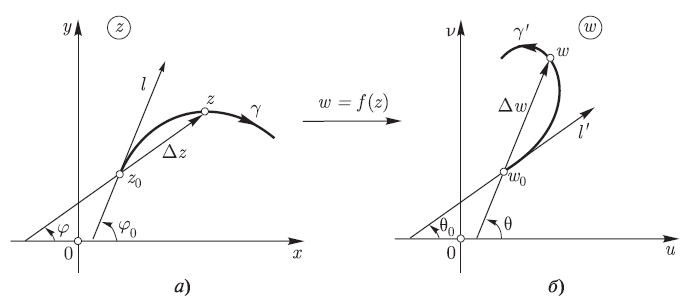
\includegraphics[keepaspectratio]{Вопросы/media/Pasted image 20260605234927.png}}

При отображении \(w = f(z)\) касательная \(l\) к кривой \(\gamma\) в
точке \(z_0\) переходит в касательную \(l'\) к образу \(\gamma'\) в
точке \(w_0 = f(z_0)\), повёрнутую на угол \(\arg f'(z_0)\). Здесь
\(\theta_{0}\) --- угол наклона \(l'\), \(\varphi_{0}\) --- угол наклона
\(l\) (на рисунке), откуда \(\arg f'(z_0) = \theta_{0} - \varphi_{0}\).

\newpage

\section{Определение однолистной функции, конформного отображения.
Свойства конформных
отображений.}\label{ux43eux43fux440ux435ux434ux435ux43bux435ux43dux438ux435-ux43eux434ux43dux43eux43bux438ux441ux442ux43dux43eux439-ux444ux443ux43dux43aux446ux438ux438-ux43aux43eux43dux444ux43eux440ux43cux43dux43eux433ux43e-ux43eux442ux43eux431ux440ux430ux436ux435ux43dux438ux44f.-ux441ux432ux43eux439ux441ux442ux432ux430-ux43aux43eux43dux444ux43eux440ux43cux43dux44bux445-ux43eux442ux43eux431ux440ux430ux436ux435ux43dux438ux439.}

\textbf{Определение:} \(w=f(z)\) \emph{однолистная} на \(G\), если
\(\forall z_{1},z_{2}\in G, \ z_{1}\neq z_{2}\implies f(z_{1})\neq f(z_{2})\)

\textbf{Определение:} Отображение, осуществляемое функцией
\(w=f(z), z\in G\), называется \emph{конформным}, если удовлетворяет
условиям:

\begin{enumerate}
\def\labelenumi{\arabic{enumi}.}
\tightlist
\item
  \(f(z)\) аналитическая в \(G\);
\item
  \(f(z)\) однолистная функция;
\item
  \(f'(z)\neq 0\quad\forall z\in G\)
\end{enumerate}

\textbf{Свойства конформных отображений:}

\begin{enumerate}
\def\labelenumi{\arabic{enumi}.}
\tightlist
\item
  При конформным отображении \(w=f(z)\) образом области \(G\) является
  область расширенной комплексной области плоскости \(w\).
\item
  Отображение, обратное к конформному отображению, также является
  конформным.
\item
  Суперпозиция (последовательное выполнение) конформных отображений
  также является конформным
\item
  При конформном отображении \(w=f(z)\) области \(G\) в каждой конечной
  точке \(z_{0}\in G\) \emph{линейное растяжение} одинаково для всех
  гладких кривых с началом в точке \(z_{0}\) и равно \(|f'(z_{0})|\),
  т.е. \emph{образом окружности} \(|z-z_{0}|=\rho\) с точностью до
  \(o(\rho)\) является \emph{окружность} \(|w-w_{0}|=\rho |f'(z_{0})|\),
  где \(w_{0}=f(z_{0})\)
\item
  При конформном отображении \(w=f(z)\) области \(G\) углы между кривыми
  с началом в точке \(z_{0}\in G, z_{0}\neq \infty\), или с концом в
  точке \(z_{0}=\infty\) равен углу между образами этих кривых в точке
  \(w_{0}=f(z_{0})\); при этом если \(z_{0}\neq \infty\), то угол
  поворота всех кривых с началом в точке \(z_{0}\) равен
  \(\arg f'(z_{0})\).
\end{enumerate}

\newpage

\section{Определение дробно-линейной функции. Отображение прямых и
окружностей при дробно-линейном отображении. Выражение для
дробно-линейной функции, отображающей три заданные точки комплексной
плоскости в три заданные
точки.}\label{ux43eux43fux440ux435ux434ux435ux43bux435ux43dux438ux435-ux434ux440ux43eux431ux43dux43e-ux43bux438ux43dux435ux439ux43dux43eux439-ux444ux443ux43dux43aux446ux438ux438.-ux43eux442ux43eux431ux440ux430ux436ux435ux43dux438ux435-ux43fux440ux44fux43cux44bux445-ux438-ux43eux43aux440ux443ux436ux43dux43eux441ux442ux435ux439-ux43fux440ux438-ux434ux440ux43eux431ux43dux43e-ux43bux438ux43dux435ux439ux43dux43eux43c-ux43eux442ux43eux431ux440ux430ux436ux435ux43dux438ux438.-ux432ux44bux440ux430ux436ux435ux43dux438ux435-ux434ux43bux44f-ux434ux440ux43eux431ux43dux43e-ux43bux438ux43dux435ux439ux43dux43eux439-ux444ux443ux43dux43aux446ux438ux438-ux43eux442ux43eux431ux440ux430ux436ux430ux44eux449ux435ux439-ux442ux440ux438-ux437ux430ux434ux430ux43dux43dux44bux435-ux442ux43eux447ux43aux438-ux43aux43eux43cux43fux43bux435ux43aux441ux43dux43eux439-ux43fux43bux43eux441ux43aux43eux441ux442ux438-ux432-ux442ux440ux438-ux437ux430ux434ux430ux43dux43dux44bux435-ux442ux43eux447ux43aux438.}

\textbf{Определение:} \emph{Дробно-линейной} называется функция \[
w= \frac{az+b}{cz+d},\quad ad-bc\neq 0,\quad(1)
\] где \(a,b,c,d\) - заданные комплексные числа. Условие \(ad-bc\neq 0\)
означает, что \(w\not\equiv \mathrm{const}\). Отображение,
осуществляемое функцией (1) называется \emph{дробно-линейным}. При этом
предполагается, что если \(c\neq 0\), то
\(w\left( -\dfrac{d}{c} \right)=\infty,w(\infty)= \dfrac{a}{c}\), а если
\(c=0\), то \(w(\infty)=\infty\). В частности, если \(c=0\), то функция
(1) является линейной, а отображение, осуществляемое линейной функцией,
называется \emph{линейным}.

\textbf{Теорема:} При дробно-линейном отображении образом любой
окружности или прямой является окружность или прямая.

\textbf{Теорема:} Существует единственное дробно-линейное отображение,
при котором три различные точки \(z_{1},z_{2},z_{3}\) переходят
соответственно в три различные точки \(w_{1},w_{2},w_{3}\). Это
отображение определяется формулой \[
\frac{w-w_{1}}{w-w_{2}}\cdot \frac{w_{3}-w_{2}}{w_{3}-w_{1}}= \frac{z-z_{1}}{z-z_{2}}\cdot \frac{z_{3}-z_{2}}{z_{3}-z_{1}}
\]

\newpage

\section{Определение интеграла от функции комплексного переменного по
ориентированному контуру. Свойства интеграла от функции комплексного
переменного.}\label{ux43eux43fux440ux435ux434ux435ux43bux435ux43dux438ux435-ux438ux43dux442ux435ux433ux440ux430ux43bux430-ux43eux442-ux444ux443ux43dux43aux446ux438ux438-ux43aux43eux43cux43fux43bux435ux43aux441ux43dux43eux433ux43e-ux43fux435ux440ux435ux43cux435ux43dux43dux43eux433ux43e-ux43fux43e-ux43eux440ux438ux435ux43dux442ux438ux440ux43eux432ux430ux43dux43dux43eux43cux443-ux43aux43eux43dux442ux443ux440ux443.-ux441ux432ux43eux439ux441ux442ux432ux430-ux438ux43dux442ux435ux433ux440ux430ux43bux430-ux43eux442-ux444ux443ux43dux43aux446ux438ux438-ux43aux43eux43cux43fux43bux435ux43aux441ux43dux43eux433ux43e-ux43fux435ux440ux435ux43cux435ux43dux43dux43eux433ux43e.}

\textbf{Кривые:}

\begin{itemize}
\tightlist
\item
  \(\gamma:\begin{cases}x=x(t) \\ y=y(t)\end{cases}, \ t\in[\alpha;\beta], \ x(t),y(t)\in C^{1}[\alpha;\beta]\)
  - уравнение гладкой кривой;
\item
  \(\gamma:x(\alpha)=x(\beta), \ y(\alpha)=y(\beta)\) - замкнутая кривая
\item
  \(\gamma:\) Кривая Жордана: из
  \(t_{1}\neq t_{2}\in[\alpha;\beta)\implies(x(t_{1}),y(t_{1}))\neq(x(t_{2}),y(t_{2}))\)
  - простая кривая
\item
  \(\gamma:\) ориентированная кривая:

  \begin{itemize}
  \tightlist
  \item
    указание на начало и конец \(\gamma\) (незамкнутая кривая)
  \item
    направление обхода границы области \(G: \ \gamma=\partial G\)
  \item
    по возрастанию параметр \(t\)
  \end{itemize}
\end{itemize}

\textbf{Определение:} Интеграл функции \(f(z)\) по \(\gamma:\)

\begin{enumerate}
\def\labelenumi{\arabic{enumi}.}
\tightlist
\item
  \(p\) - разбиение \([\alpha;\beta]\), \(t=\{ t_{i} \}_{i=1}^{n}\) -
  точки разбиения \(p\), \(\Delta t_{i}=t_{i}-t_{i-1}\) - отрезок,
  \(L(p)=\max\limits_{i\in \{ 1,\dots,n \}}\Delta t_{i}\) - мелкость
  разбиения, набор \(\xi=\{ \xi_{i} \}_{i=1}^{n}\) - выборка из
  разбиения \(p\), если
  \(\forall i=\overline{1,n}\quad \xi_{i}\in H_{i}:=[t_{i-1},t_{i}]\)
\item
  \(\Delta z_{i}=z(t_{i})- z(t_{i-1}), \ z=z(t)\) - уравнение
  \(\gamma, \ |\Delta z_{i}|=|\Delta l_{i}|\)
\item
  \(\sigma(f,p,\xi)=\sum\limits_{i=1}^{n}f(z(\xi_{i}))\cdot\Delta z_{i}\)
  - интегральная сумма
\end{enumerate}

\textbf{Определение:} Интегралом функции \(f(z)\) по \(\gamma\),
обозначение \(I=\int\limits_{\gamma}f(z)\,dz\), называют число
\(I\in \mathbb{C}: \ \lim_{ L(p) \to 0}\sigma(f,p,\xi)=I\): \[
\forall\varepsilon>0 \ \exists\delta>0 \forall p \in P_{\delta} \ \forall \xi \in V_{p}\implies |\sigma(f,p,\xi)-I|<\varepsilon
\]

Функция называется интегрируемой на \(\gamma\), если
\(\exists \int\limits_{\gamma}f(z)\,dz\).

\textbf{Свойства:}

\begin{enumerate}
\def\labelenumi{\arabic{enumi}.}
\tightlist
\item
  Линейность \(\forall f(z), g(z)\) - интегрируемые функции на
  \(\gamma\), \(\forall\lambda,\mu \in \mathbb{C}\). Тогда \[
  \int_{\gamma}(\lambda\cdot f(z)+\mu\cdot g(z))\,dz=\lambda \int_{\gamma}f(z)\,dz+\mu \int_{\gamma}g(z)\,dz
  \]
\item
  \(\gamma^{+}\) и \(\gamma^{-}\) - кривые с разной ориентацией,
  \(f(z)\) - интегрируемая функция на \(\gamma^{+}, \gamma^{-}\): \[
  \int_{\gamma^{+}}f(z)\,dz=-\int_{\gamma^{-}}f(z)\,dz
  \]
\item
  Аддитивность интеграла по множеству:
  \(\gamma=\gamma_{1}\cup\gamma_{2}, \ f(z)\) интегрируема на
  \(\gamma_{1}\) и \(\gamma_{2}\). Тогда \[
  \int_{\gamma_{1}\cup\gamma_{2}}f(z)\,dz=\int_{\gamma_{1}}f(z)\,dz+\int_{\gamma_{2}}f(z)\,dz
  \]
\item
  Оценка интеграла: \(\gamma:z=z(t), \ t\in[\alpha;\beta]\) \[
  \left\lvert \int f(z)\,dz   \right\rvert \leq \int_{\gamma} |f(z)|\,d\ell \overset{\mathrm{def}}{=}\int_{\gamma}|f(z)|\,|dz|,
  \] где
  \(d \ell=\sqrt{ x'^{2}(t)+y'^{2}(t) }\,dt=|z'(t)|\,dt=|z'(t)\,dt|=|dz|\)
\item
  Если ряд \(f(z)=\sum\limits_{n=1}^{\infty}f_{n}(z)\), составленный из
  непрерывных на кривой \(\gamma\) функций \(f_{n}(z)\)
  \((n=1,2,\dots)\), сходится равномерно на \(\gamma\), то его можно
  почленно интегрировать, т.е. \[
  \int_{\gamma}f(z)\,dz=\sum_{n=1}^{\infty}\int_{\gamma}f_{n}(z)\,dz.
  \]
\end{enumerate}

\newpage

\section{Интегральная формула Коши для функции и для производной
функции.}\label{ux438ux43dux442ux435ux433ux440ux430ux43bux44cux43dux430ux44f-ux444ux43eux440ux43cux443ux43bux430-ux43aux43eux448ux438-ux434ux43bux44f-ux444ux443ux43dux43aux446ux438ux438-ux438-ux434ux43bux44f-ux43fux440ux43eux438ux437ux432ux43eux434ux43dux43eux439-ux444ux443ux43dux43aux446ux438ux438.}

\textbf{Теорема:} Пусть

\begin{enumerate}
\def\labelenumi{\arabic{enumi}.}
\tightlist
\item
  \(G\) - область на \(\mathbb{C}\) с кусочно-гладкой границей;
\item
  \(\partial G\) ориентирована положительно относительно G;
\item
  \(f(z)\) - аналитическая функция на \(G\);
\item
  \(f(z)\) - непрерывная на \(\overline{G}\). Тогда \(\forall z\in G\)
  справедливо равенство \[
  f(z)= \frac{1}{2\pi i}\int_{\partial G} \frac{f(\xi)\,d\xi}{\xi-z}
  \]
\end{enumerate}

\textbf{Теорема:} Пусть

\begin{enumerate}
\def\labelenumi{\arabic{enumi}.}
\tightlist
\item
  \(G\) - область на \(\mathbb{C}\) с кусочно-гладкой границей;
\item
  \(\partial G\) ориентирована положительно относительно G;
\item
  \(f(z)\) - аналитическая функция на \(G\);
\item
  \(f(z)\) - непрерывная на \(\overline{G}\). Тогда \(\forall z\in G\)
  функция \(f(z)\) имеет производные всех порядков в точке \(z\),
  вычисляемые по формуле: \[
  f^{(n)}(z)= \frac{n!}{2\pi i}\int_{\partial G} \frac{f(\xi)}{(\xi-z)^{n+1}}\,d\xi, \ n=1,2,\dots
  \]
\end{enumerate}

\newpage

\section{Определение первообразной функции комплексного переменного.
Теорема о достаточных условиях существования первообразной. Теорема о
формуле Ньютона -Лейбница в случае комплексного
переменного.}\label{ux43eux43fux440ux435ux434ux435ux43bux435ux43dux438ux435-ux43fux435ux440ux432ux43eux43eux431ux440ux430ux437ux43dux43eux439-ux444ux443ux43dux43aux446ux438ux438-ux43aux43eux43cux43fux43bux435ux43aux441ux43dux43eux433ux43e-ux43fux435ux440ux435ux43cux435ux43dux43dux43eux433ux43e.-ux442ux435ux43eux440ux435ux43cux430-ux43e-ux434ux43eux441ux442ux430ux442ux43eux447ux43dux44bux445-ux443ux441ux43bux43eux432ux438ux44fux445-ux441ux443ux449ux435ux441ux442ux432ux43eux432ux430ux43dux438ux44f-ux43fux435ux440ux432ux43eux43eux431ux440ux430ux437ux43dux43eux439.-ux442ux435ux43eux440ux435ux43cux430-ux43e-ux444ux43eux440ux43cux443ux43bux435-ux43dux44cux44eux442ux43eux43dux430--ux43bux435ux439ux431ux43dux438ux446ux430-ux432-ux441ux43bux443ux447ux430ux435-ux43aux43eux43cux43fux43bux435ux43aux441ux43dux43eux433ux43e-ux43fux435ux440ux435ux43cux435ux43dux43dux43eux433ux43e.}

\textbf{Определение:} Функция \(F(z)\) называется \emph{первообразной
функции} \(f(z)\), определенной в области \(G\), если функция \(F(z)\)
определена в области \(G\), дифференцируема в этой области и \[
F'(z)=f(z),\quad z\in G
\]

\textbf{Теорема:} (Теорема о достаточных условиях существования
первообразной) Пусть

\begin{enumerate}
\def\labelenumi{\arabic{enumi}.}
\tightlist
\item
  \(f(z)\in C(G)\);
\item
  \(\forall\) замкнутого контура \(\gamma \in G\) выполняется условие
  \(\int\limits_{\gamma}f(z)\,dz=0\) Тогда \(f(z)\) имеет первообразную
  в \(G\).
\end{enumerate}

\textbf{Теорема:} (Теорема о формуле Ньютона-Лейбница в случае
комплексного переменного) Пусть

\begin{enumerate}
\def\labelenumi{\arabic{enumi}.}
\tightlist
\item
  \(f\in C(G), G\subset \mathbb{C}\)
\item
  \(\exists F(z)\) - первообразная функции \(f(z)\) в \(G\)
\item
  \(\gamma_{b,c}\) - любой путь (кусочно-гладкий), соединяющий точки
  \(b,c\in G\)
  (\(\gamma_{b,c}=\gamma_{b,c}(t), t\in[\alpha;\beta ], \ \gamma_{b,c}(t)\in C^{1}_{\text{кус.}}[\alpha;\beta], \ \gamma_{b,c}(\alpha)=b, \ \gamma_{b,c}(\beta)=c\))
  \[
  \int\limits_{\gamma_{b,c}}f(z)\,dz=F(c)-F(b),
  \]
\end{enumerate}

\newpage

\input{tex/18.tex}
\newpage

\section{Классификация (определения) изолированных особых точек
аналитических функций. Теорема о структуре главной и правильной частей
ряда Лорана в кольце, центр которого совпадает с изолированной особой
точкой
функции.}\label{ux43aux43bux430ux441ux441ux438ux444ux438ux43aux430ux446ux438ux44f-ux43eux43fux440ux435ux434ux435ux43bux435ux43dux438ux44f-ux438ux437ux43eux43bux438ux440ux43eux432ux430ux43dux43dux44bux445-ux43eux441ux43eux431ux44bux445-ux442ux43eux447ux435ux43a-ux430ux43dux430ux43bux438ux442ux438ux447ux435ux441ux43aux438ux445-ux444ux443ux43dux43aux446ux438ux439.-ux442ux435ux43eux440ux435ux43cux430-ux43e-ux441ux442ux440ux443ux43aux442ux443ux440ux435-ux433ux43bux430ux432ux43dux43eux439-ux438-ux43fux440ux430ux432ux438ux43bux44cux43dux43eux439-ux447ux430ux441ux442ux435ux439-ux440ux44fux434ux430-ux43bux43eux440ux430ux43dux430-ux432-ux43aux43eux43bux44cux446ux435-ux446ux435ux43dux442ux440-ux43aux43eux442ux43eux440ux43eux433ux43e-ux441ux43eux432ux43fux430ux434ux430ux435ux442-ux441-ux438ux437ux43eux43bux438ux440ux43eux432ux430ux43dux43dux43eux439-ux43eux441ux43eux431ux43eux439-ux442ux43eux447ux43aux43eux439-ux444ux443ux43dux43aux446ux438ux438.}

\textbf{Определение:} Точка \(z=a\in \overline{\mathbb{C}}\) называется
\emph{изолированной} особой точкой, если

\begin{enumerate}
\def\labelenumi{\arabic{enumi}.}
\tightlist
\item
  в \(z=a\) функция не является аналитической;
\item
  \(\exists K_{0,\rho}=\dot{U}_{\rho}(a)\), в котором \(f(z)\) -
  аналитическая В частности, \(a=\infty\), то 2. аналитичность в
  \(U_{\rho}(\infty)=\{ z\in \mathbb{C}: |z|>\rho \}\) (изолированная
  точка \(a=\infty\)).
\end{enumerate}

\textbf{Определение:} Точка \(z=a\) - \emph{устранимая} особая точка
функции \(f(z)\), если \(\exists \lim_{ z \to a }f(z)=A<\infty\) (в
частности, \(a=\infty \ \exists \lim_{ z \to \infty }f(z)=A<\infty\))

\textbf{Определение:} Точка \(z=a\) - \emph{полюс порядка \(m\)} функции
\(f(z)\), если

\begin{enumerate}
\def\labelenumi{\arabic{enumi}.}
\tightlist
\item
  \(\exists \lim_{ z \to a }f(z)=\infty\)
\item
  \(\exists \lim_{ z \to a }(z-a)^{m}\cdot f(z)=B<\infty\) (в частности,
  \(a=\infty\), то 1. \(\exists \lim_{ z \to \infty }f(z)=\infty,\) 2.
  \(\exists \lim_{ z \to \infty } \dfrac{f(z)}{z^{m}}=B<\infty\))
\end{enumerate}

\textbf{Определение:} Точка \(z=a\) - \emph{существенная} особая точка
функции \(f(z)\), если у нее не существует предела(ни конечного, ни
бесконечного).

\[
a\neq \infty: f(z)=\underbrace{\sum_{n=-\infty}^{-1}c_{n}(z-a)^{n}}_{f_{1}(z) - \text{главная часть}}+\underbrace{\sum_{n=0}^{+\infty}c_{n}(z-a)^{n}}_{f_{2}(z) - \text{правильная часть}}\quad \begin{array}{l} 
\lim_{ z \to a }f_{2}(z)=B<\infty \\
\lim_{ z \to a }f_{1}(z)=\infty  \end{array}
\] \[
a=\infty: f(z)=\underbrace{\sum_{n=-\infty}^{-1}c_{n}\cdot z^{n}}_{f_{1}(z) - \text{правильная часть}}+\underbrace{\sum_{n=0}^{+\infty}c_{n}\cdot z^{n}}_{f_{2}(z) - \text{главная часть}}\quad \begin{array}{l}  \lim_{ z \to \infty }f_{2}(z)=\infty \\
\lim_{ z \to \infty }f_{1}(z)=0  \end{array}
\]

\textbf{Теорема:} Пусть \(z=a\in \overline{\mathbb{C}}\) - изолированная
особая точка функций \(f(z)\)

\begin{itemize}
\tightlist
\item
  Точка \(z=a\) - устранимая особая точка в том и только в том случае,
  если у ряда Лорана функции \(f(z)\) отсутствует главная часть.
\item
  Точка \(z=a\) - полюс порядка \(m\) функции \(f(z)\) в том и только в
  том случае, если главная часть ряда Лорана содержит конечное число
  членов: \[
  c_{-n}=0 \ \forall n>m\text{ и } c_{-m}\neq 0
  \] (для \(a=\infty\) главная часть содержит конечное число членов:
  \(c_{n}=0, \forall n>m, c_{m}\neq 0\))
\item
  Точка \(z=a\) - существенно особая точка функции \(f(z)\) в том и
  только в том случае, если главная часть ряда Лорана содержит
  \(\infty\) число членов.
\end{itemize}

\newpage

\section{\texorpdfstring{Понятие вычета аналитической функции в её
изолированной особой точке. Формула для нахождения вычета в полюсе
порядка \(m \in \mathbb{N}\). Вычет функции в точке
\(z=\infty\).}{Понятие вычета аналитической функции в её изолированной особой точке. Формула для нахождения вычета в полюсе порядка m \textbackslash in \textbackslash mathbb\{N\}. Вычет функции в точке z=\textbackslash infty.}}\label{ux43fux43eux43dux44fux442ux438ux435-ux432ux44bux447ux435ux442ux430-ux430ux43dux430ux43bux438ux442ux438ux447ux435ux441ux43aux43eux439-ux444ux443ux43dux43aux446ux438ux438-ux432-ux435ux451-ux438ux437ux43eux43bux438ux440ux43eux432ux430ux43dux43dux43eux439-ux43eux441ux43eux431ux43eux439-ux442ux43eux447ux43aux435.-ux444ux43eux440ux43cux443ux43bux430-ux434ux43bux44f-ux43dux430ux445ux43eux436ux434ux435ux43dux438ux44f-ux432ux44bux447ux435ux442ux430-ux432-ux43fux43eux43bux44eux441ux435-ux43fux43eux440ux44fux434ux43aux430-m-in-mathbbn.-ux432ux44bux447ux435ux442-ux444ux443ux43dux43aux446ux438ux438-ux432-ux442ux43eux447ux43aux435-zinfty.}

Пусть \(a\in \overline{\mathbb{C}}\) - изолированная особая точка
\(\Leftrightarrow \exists \dot{U}_{\rho}(a)\), в которой \(f(z)\)
аналитическая. Если \(a=\infty\), то
\(U_{\rho}=\{ z\in \mathbb{C}:|z|>\rho \}\) - окрестность бесконечности.

\textbf{Определение:} \emph{Вычетом} функции \(f(z)\) в точке \(a\),
обозначим \(\underset{a}{\mathrm{res}} f\), называется число \[
\frac{1}{2\pi i}\int_{\gamma_{r}^{+}(a)}f(z)\,dz=\underset{a}{\mathrm{res}} f, \ 0<r<\rho, \forall r
\] (не зависит от \(r\)).

\textbf{Замечание:} \[
\underset{a}{\mathrm{res}} f=c_{-1}
\]

\textbf{Теорема:} Формула для нахождения вычета в полюсе порядка
\(m\in \mathbb{N}\): Пусть \(a\) - полюс порядка \(m\in \mathbb{N}\).
Тогда \(\underset{a}{\mathrm{res}} f\) равен: \[
\underset{a}{\mathrm{res}}f=  \frac{1}{(m-1)!}\cdot \lim_{ z \to a }  \frac{d^{m-1}}{(dz)^{m-1}}((z-a)^{m}\cdot f(z))
\]

Вычеты в точке \(z=a=\infty\) \(\to\) \(f(z)\) аналитическая в
\(U_{\rho}(\infty)=\{ z\in \mathbb{C}:|z|>\rho \}\) - Кольцо
\(K_{\rho,\infty}(0)\implies\) ряд Лорана в точке \(a=\infty\): \[
f(z)=\sum_{n=-\infty}^{+\infty}c_{n}z^{n},
\] где
\(c_{n}= \dfrac{1}{2\pi i}\int\limits_{\gamma_{r}(0)} \dfrac{f(z)}{z^{n+1}}\,dz, \forall r>\rho\)

\textbf{Определение:} Вычетом функции \(f(z)\) в точке \(z=a=\infty\),
обозначим \(\underset{\infty}{\mathrm{res}}f\), называют число, равное:
\[
\frac{1}{2\pi i}\int_{\gamma_{r}^{-}(0)}f(z)\,dz=\underset{\infty}{\mathrm{res}} f
\]

\textbf{Замечание:} \[
\underset{\infty}{\mathrm{res}} f=-c_{-1}
\]

\textbf{Формула:} Для \(\underset{\infty}{\mathrm{res}} f\), если
\(a=\infty\) - особая устранимая точка: \[
\underset{\infty}{\mathrm{res}} f=\lim_{ z \to \infty } (z\cdot(f(\infty)-f(z)))
\]

\newpage

\section{\texorpdfstring{Теорема Коши о вычетах. Теорема о равенстве
нулю суммы вычетов функции, аналитической на всей комплексной плоскости,
за исключением конечного числа её изолированных особых точек, включая
\(z=\infty\).}{Теорема Коши о вычетах. Теорема о равенстве нулю суммы вычетов функции, аналитической на всей комплексной плоскости, за исключением конечного числа её изолированных особых точек, включая z=\textbackslash infty.}}\label{ux442ux435ux43eux440ux435ux43cux430-ux43aux43eux448ux438-ux43e-ux432ux44bux447ux435ux442ux430ux445.-ux442ux435ux43eux440ux435ux43cux430-ux43e-ux440ux430ux432ux435ux43dux441ux442ux432ux435-ux43dux443ux43bux44e-ux441ux443ux43cux43cux44b-ux432ux44bux447ux435ux442ux43eux432-ux444ux443ux43dux43aux446ux438ux438-ux430ux43dux430ux43bux438ux442ux438ux447ux435ux441ux43aux43eux439-ux43dux430-ux432ux441ux435ux439-ux43aux43eux43cux43fux43bux435ux43aux441ux43dux43eux439-ux43fux43bux43eux441ux43aux43eux441ux442ux438-ux437ux430-ux438ux441ux43aux43bux44eux447ux435ux43dux438ux435ux43c-ux43aux43eux43dux435ux447ux43dux43eux433ux43e-ux447ux438ux441ux43bux430-ux435ux451-ux438ux437ux43eux43bux438ux440ux43eux432ux430ux43dux43dux44bux445-ux43eux441ux43eux431ux44bux445-ux442ux43eux447ux435ux43a-ux432ux43aux43bux44eux447ux430ux44f-zinfty.}

\textbf{Теорема} (Теорема Коши о вычетах) Пусть

\begin{enumerate}
\def\labelenumi{\arabic{enumi}.}
\tightlist
\item
  Область \(G\subset \overline{\mathbb{C}}\) (возможно
  \(a=\infty \in G\) вместе с окрестностью \(U_{r}(\infty)\)) с
  кусочно-гладкой границей \(\partial G\) (возможно многосвязная)
\item
  Функция \(f(z)\) аналитическая в \(G\) за исключением конечного числа
  изолированных особых точек \(a_{1},a_{2},\dots,a_{m-1},a_{m}=\infty\)
  (возможно)
\item
  Функция \(f(z)\) непрерывна в \(G\) вплоть до границы \(\partial G\).
  Тогда справедлива формула: \[
  \int_{\partial G}f(z)\,dz=2\pi i \sum_{k=1}^{m}\underset{a_{k}}{\mathrm{res}} f
  \]
\end{enumerate}

\textbf{Теорема:} Пусть
\(G=\overline{\mathbb{C}}\setminus \{ a_{1},a_{2},\dots,a_{m}=\infty \}\)
и функция \(f(z)\) аналитическая на всей расширенной комплексной
плоскости за исключением конечного числа изолированных особых точек.
Тогда \[
\sum_{k=1}^{m}\underset{a_{k}}{\mathrm{res}} f=0
\]

\newpage

\input{tex/22.tex}
\newpage

\section{Определение оригинала и изображения по Лапласу. Теорема о
существовании изображения и его
аналитичности.}\label{ux43eux43fux440ux435ux434ux435ux43bux435ux43dux438ux435-ux43eux440ux438ux433ux438ux43dux430ux43bux430-ux438-ux438ux437ux43eux431ux440ux430ux436ux435ux43dux438ux44f-ux43fux43e-ux43bux430ux43fux43bux430ux441ux443.-ux442ux435ux43eux440ux435ux43cux430-ux43e-ux441ux443ux449ux435ux441ux442ux432ux43eux432ux430ux43dux438ux438-ux438ux437ux43eux431ux440ux430ux436ux435ux43dux438ux44f-ux438-ux435ux433ux43e-ux430ux43dux430ux43bux438ux442ux438ux447ux43dux43eux441ux442ux438.}

\textbf{Определение:} \emph{Оригиналом} называют комплекснозначную
функцию \(f(t)\) действительного переменного \(t\), если:

\begin{enumerate}
\def\labelenumi{\arabic{enumi}.}
\tightlist
\item
  \(f(t)=0\) при \(t<0\)
\item
  на каждом отрезке полуоси \(t\geq 0\) функция \(f(t)\) непрерывна,
  кроме, быть может, конечного числа точек разрыва первого рода;
\item
  Существуют такие действительные числа \(M>0\) и \(\alpha\), что
  \(\forall t\geq 0\) выполняется неравенство: \[
  |f(t)|\leq Me^{ \alpha t }
  \]
\end{enumerate}

\textbf{Определение:} \emph{Изображением} оригинала \(f(t)\) называют
комплекснозначную функцию \[
F(p)=\int_{0}^{+\infty}e^{ -pt }\cdot f(t)\,dt\quad(2)
\] комплексного переменного \(p\).

\textbf{Определение:} Интеграл (2) называют \emph{преобразованием
Лапласа} функции \(f(t)\).

Связь между оригиналом \(f(t)\) и его изображением \(F(p)\) записывают
так: \[
f(t)\risingdotseq F(p)\text{ или }F(p)\risingdotseq f(t)
\] \textbf{Теорема:} Пусть \(f(t)\) - оригинал. Тогда \(f(t)\) имеет
изображение \(F(p)=\int_{0}^{\infty}f(t)e^{ -pt }\,dt\) и \(F(p)\) -
аналитическая функция в области
\(G_{\alpha}=\{ p\in \mathbb{C}: \mathrm{Re}p>\alpha \}\).

\newpage

\section{Свойства преобразования Лапласа: подобие, сдвиг изображения,
запаздывание
оригинала.}\label{ux441ux432ux43eux439ux441ux442ux432ux430-ux43fux440ux435ux43eux431ux440ux430ux437ux43eux432ux430ux43dux438ux44f-ux43bux430ux43fux43bux430ux441ux430-ux43fux43eux434ux43eux431ux438ux435-ux441ux434ux432ux438ux433-ux438ux437ux43eux431ux440ux430ux436ux435ux43dux438ux44f-ux437ux430ux43fux430ux437ux434ux44bux432ux430ux43dux438ux435-ux43eux440ux438ux433ux438ux43dux430ux43bux430.}

\textbf{Подобие:} Если \(f(t)\risingdotseq F(p)\) и \(\beta>0\), то \[
f(\beta t)\risingdotseq \frac{1}{\beta}F\left( \frac{p}{\beta} \right)
\] \textbf{Сдвиг изображения:} Если \(f(t)\risingdotseq F(p)\), то
\(\forall a\in \mathbb{C}:\) \[
f(t)e^{ a t }\risingdotseq F(p-a)
\]

\textbf{Запаздывание оригинала:} Если \(f(t)\risingdotseq F(p)\) и
\(f(t)=0\) при \(t<\tau\), где \(\tau>0\), то \[
f(t-\tau)\risingdotseq e^{ -p\tau }F(p).
\]

\newpage

\section{Дифференцирование оригинала, дифференцирование изображения,
изображение
свёртки.}\label{ux434ux438ux444ux444ux435ux440ux435ux43dux446ux438ux440ux43eux432ux430ux43dux438ux435-ux43eux440ux438ux433ux438ux43dux430ux43bux430-ux434ux438ux444ux444ux435ux440ux435ux43dux446ux438ux440ux43eux432ux430ux43dux438ux435-ux438ux437ux43eux431ux440ux430ux436ux435ux43dux438ux44f-ux438ux437ux43eux431ux440ux430ux436ux435ux43dux438ux435-ux441ux432ux451ux440ux442ux43aux438.}

\textbf{Дифференцирование оригинала:} Если
\(f(t), f'(t),\dots,f^{(n)}(t)\) - оригиналы и
\(f(t)\risingdotseq F(p)\), то \[
f^{(n)}(t)\risingdotseq p^{n}F(p)-\sum_{k=0}^{n-1}p^{n-1-k}f^{(k)}(0),
\] где
\(f^{(k)}(0)=\lim\limits_{ t \to +0 }f^{(k)}(t), \ k=\overline{0,n-1}\).

\textbf{Дифференцирование изображения:} Если \(F(p)\risingdotseq f(t)\),
то \[
F^{(n)}(p)\risingdotseq(-t)^{n}f(t).
\] \textbf{Определение:} Если \(f(t)\) и \(g(t)\) - оригиналы, \(F(p)\)
и \(G(p)\) - их изображения, то

\begin{enumerate}
\def\labelenumi{\arabic{enumi}.}
\tightlist
\item
  функция \((f*g)(t)=\int_{0}^{t}f(\tau)g(t-\tau)\,d\tau\) называется
  \emph{свёрткой} функции \(f(t)\) и \(g(t)\);
\item
  \((f*g)(t)\) является оригиналом;
\item
  \((f*g)(t)=(g*f)(t)\) - коммутативность свёртки;
\item
  \((f*g)(t)\risingdotseq F(p)\cdot G(p)\).
\end{enumerate}

\newpage

\section{Интегрирование оригинала, интегрирование
изображения.}\label{ux438ux43dux442ux435ux433ux440ux438ux440ux43eux432ux430ux43dux438ux435-ux43eux440ux438ux433ux438ux43dux430ux43bux430-ux438ux43dux442ux435ux433ux440ux438ux440ux43eux432ux430ux43dux438ux435-ux438ux437ux43eux431ux440ux430ux436ux435ux43dux438ux44f.}

\textbf{Интегрирование оригинала:} Если \(f(t)\risingdotseq F(p)\), то
\[
\int_{0}^{t}f(\tau)\,d\tau\risingdotseq \frac{F(p)}{p}
\]

\textbf{Интегрирование изображения:} Если \(f(t)\risingdotseq F(p)\) и
\(\dfrac{1}{t}f(t)\) - оригинал, то \[
\frac{1}{t}f(t)\risingdotseq\int_{p}^{\infty}F(\zeta)\,d\zeta,
\] где \((p,\infty)\) - горизонтальный луч, принадлежащий полуплоскости
\(\mathrm{Re} p>\alpha\), от точки \(p\) до точки
\(\mathrm{Re}p=+\infty\).


\end{document}
    